\documentclass[10pt,border=5pt]{standalone}
\usepackage[T1]{fontenc}
\usepackage{lmodern,amsmath,amssymb,mathrsfs,tikz}
\usetikzlibrary{arrows.meta,positioning,calc}
\definecolor{ink}{HTML}{192536}
\definecolor{blue}{HTML}{2E70AE}
\definecolor{gold}{HTML}{A66A15}
\definecolor{green}{HTML}{28764D}
\definecolor{red}{HTML}{B43D3D}
\newcommand{\C}{\mathbb C}
\newcommand{\R}{\mathcal R}
\newcommand{\Lr}{\mathcal L_{\mathrm{res}}}
\newcommand{\Prs}{\mathcal P_{\mathrm{res}}}
\newcommand{\Tr}{T_{\mathrm{resp}}}
\newcommand{\rr}{\rho_{\mathrm{res}}}
\tikzset{every node/.style={font=\small,text=ink,align=center},
 box/.style={draw=blue,fill=blue!4,rounded corners=3pt,line width=.7pt,inner sep=7pt},
 goldbox/.style={box,draw=gold,fill=gold!5},
 greenbox/.style={box,draw=green,fill=green!5},
 redbox/.style={box,draw=red,fill=red!4},
 edge/.style={-{Stealth[length=4pt]},draw=ink,line width=.7pt},
 heading/.style={font=\small\bfseries},
 note/.style={font=\small,text=ink!85}}

\begin{document}
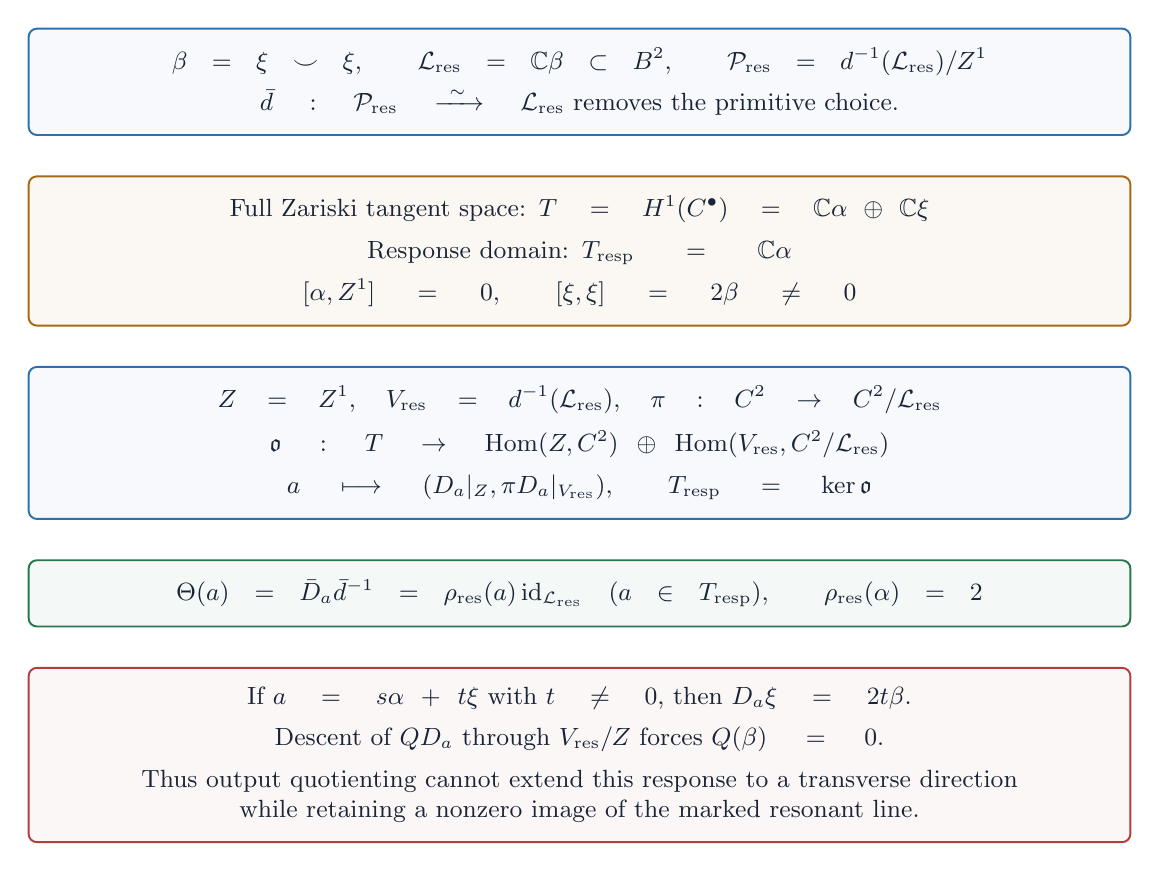
\begin{tikzpicture}
\node[box,text width=13.5cm] (pair)
 {$\beta=\xi\smile\xi,\qquad \Lr=\C\beta\subset B^2,\qquad
 \Prs=d^{-1}(\Lr)/Z^1$\\[4pt]
 $\bar d:\Prs\xrightarrow{\ \sim\ }\Lr$ removes the primitive choice.};
\node[goldbox,text width=13.5cm,below=5mm of pair] (domain)
 {Full Zariski tangent space: $T=H^1(C^\bullet)=\C\alpha\oplus\C\xi$\\[4pt]
 Response domain: $\Tr=\C\alpha$\\[4pt]
 $[\alpha,Z^1]=0,\qquad [\xi,\xi]=2\beta\ne0$};
\node[box,text width=13.5cm,below=5mm of domain] (obs)
 {$Z=Z^1,\quad V_{\mathrm{res}}=d^{-1}(\Lr),\quad
 \pi:C^2\to C^2/\Lr$\\[5pt]
 $\mathfrak o:T\to\operatorname{Hom}(Z,C^2)\oplus
 \operatorname{Hom}(V_{\mathrm{res}},C^2/\Lr)$\\[4pt]
 $a\longmapsto(D_a|_Z,\pi D_a|_{V_{\mathrm{res}}}),\qquad
 \Tr=\ker\mathfrak o$};
\node[greenbox,text width=13.5cm,below=5mm of obs] (resp)
 {$\Theta(a)=\bar D_a\bar d^{-1}=\rr(a)\operatorname{id}_{\Lr}
 \quad(a\in\Tr),\qquad\rr(\alpha)=2$};
\node[redbox,text width=13.5cm,below=5mm of resp]
 {If $a=s\alpha+t\xi$ with $t\ne0$, then $D_a\xi=2t\beta$.\\[4pt]
 Descent of $QD_a$ through $V_{\mathrm{res}}/Z$ forces $Q(\beta)=0$.\\[4pt]
 Thus output quotienting cannot extend this response to a transverse direction\\
 while retaining a nonzero image of the marked resonant line.};
\end{tikzpicture}
\end{document}
